%%% PREAMBLE - Do not touch %%%%%%%%%%%%%%%%%%%%%%%%%%%%%%%%%%%%%%%%%%%%%%%%%%%%%%
\documentclass[10pt,twocolumn,letterpaper]{article}
\usepackage[utf8]{inputenc}
\usepackage[T1]{fontenc}
\usepackage[portuges,brazilian,english]{babel}
\usepackage{model}
\usepackage{times}
\usepackage{epsfig}
\usepackage{graphicx}
\usepackage{amsmath}
\usepackage{amssymb}
\usepackage{color}
\usepackage[pagebackref=true,breaklinks=true,letterpaper=true,colorlinks,bookmarks=false]{hyperref}
%  ABACO -- Conjunto de macros para desenhar o 'abaco
%  Desenho original de Hans Liesenberg
%  Macros de Tomasz Kowaltowski
%  DCC -- IMECC -- UNICAMP
%  Mar,co de 1988  --  Vers~ao 1.0
% Ajustado para LaTeX da SUN -- Mar,co de 1991
% ---------------------------------------------------------
%  Chamada:   \ABACO{d1}{d2}{d3}{d4}{esc}
%             com:  di's -- os quatro d'igitos;
%                   esc  -- fator de escala
% ---------------------------------------------------------
%  DEFINI,C~OES AUXILIARES
% ---------------------------------------------------------
%  Forma o d'igito pequeno (0 ou 1)

\newcommand{\ABACODP}[1]{%
%
\thicklines
%    
\begin{picture}(8,0)
    \ifcase#1{   %  caso 0
       \put(0,0)    {\line(1,0){4}}
       \multiput(5,0)(2,0){2}{\oval(2,4)}}
    \or{         %  caso 1
       \put(2,0)    {\line(1,0){4}}
       \multiput(1,0)(6,0){2}{\oval(2,4)}}
    \fi
\end{picture}
    } % \ABACODP

% Forma o d'igito grande (0 a 4)

\newcommand{\ABACODG}[1]{%
%
\thicklines
%    
\begin{picture}(14,0)
    \ifcase#1{   % caso 0
       \multiput(1,0)(2,0){5}{\oval(2,4)}}
       \put(10,0)   {\line(1,0){4}}
    \or{         % caso 1
       \multiput(1,0)(2,0){4}{\oval(2,4)}}
       \put(8,0)   {\line(1,0){4}}
       \put(13,0)   {\oval(2,4)}
    \or{         % caso 2
       \multiput(1,0)(2,0){3}{\oval(2,4)}
       \put(6,0)   {\line(1,0){4}}
       \multiput(11,0)(2,0){2}{\oval(2,4)}}
    \or{         % caso 3
       \multiput(1,0)(2,0){2}{\oval(2,4)}
       \put(4,0)   {\line(1,0){4}}
       \multiput(9,0)(2,0){3}{\oval(2,4)}}
    \or{         % caso 4
       \put(1,0)  {\oval(2,4)}}
       \put(2,0)   {\line(1,0){4}}
       \multiput(7,0)(2,0){4}{\oval(2,4)}
    \fi
\end{picture}
    } % \ABACODG
       
% Forma um d'igito (0 a 9)

\newcommand{\ABACOD}[1]{%
%
    \ifnum#1>9
       \errmessage{#1: Argumento invalido para ABACO}
    \fi
    \ifnum#1<0
       \errmessage{#1: Argumento invalido para ABACO}
    \fi
%
\begin{picture}(24,0)
%    
    \ifnum#1<5
       \put(16,0) {\ABACODP{0}}
    \else   
       \put(16,0) {\ABACODP{1}}
    \fi
%    
    \ifnum#1<5
       \put(0,0)  {\ABACODG{#1}}
    \else
       \ifcase#1\or \or \or \or
          \or  \put(0,0)  {\ABACODG{0}}
          \or  \put(0,0)  {\ABACODG{1}}
          \or  \put(0,0)  {\ABACODG{2}}
          \or  \put(0,0)  {\ABACODG{3}}
          \or  \put(0,0)  {\ABACODG{4}}
       \fi
    \fi   
\end{picture}
    } % \ABACOD
    
% -------------------------------------------------

%  DEFINI,C~AO PRINCIPAL
    
\newcommand{\ABACO}[5]{%
    \setlength{\unitlength}{#5mm}
%
    \thinlines
%   
\begin{picture}(28,25)
%   
% moldura
%
% externa
%
        \put(0,0)            {\line(0,1){25}}
        \put(0,0)            {\line(1,0){28}}
        \put(28,0)           {\line(0,1){25}}
        \put(0,25)           {\line(1,0){28}}
% interna
        \put(2,2)            {\line(0,1){21}}
        \put(26,2)           {\line(0,1){21}}
        \put(16,2)           {\line(0,1){21}}
        \put(18,2)           {\line(0,1){21}}
        \put(2,2)            {\line(1,0){14}}
%        \put(16,2)           {\line(1,-1){1}}
%        \put(17,1)           {\line(1,1){1}}
        \put(18,2)           {\line(1,0){8}}
        \put(2,23)           {\line(1,0){14}}
%        \put(16,23)          {\line(1,1){1}}
%       \put(17,24)          {\line(1,-1){1}}
        \put(18,23)          {\line(1,0){8}}
%        \put(0,0)            {\line(1,1){2}}
%        \put(0,25)           {\line(1,-1){2}}
%        \put(28,0)           {\line(-1,1){2}}
%        \put(28,25)          {\line(-1,-1){2}}
%
%   
% d'igitos
%
%   
       \put(2,20)  {\ABACOD{#1}}
       \put(2,15)  {\ABACOD{#2}}
       \put(2,10)  {\ABACOD{#3}}
       \put(2,5)   {\ABACOD{#4}}
%      
\end{picture}
    } % \ABACO
    


\cvprfinalcopy % *** Uncomment this line for the final submission
\def\httilde{\mbox{\tt\raisebox{-.5ex}{\symbol{126}}}}
\ifcvprfinal\pagestyle{empty}\fi

\newcommand{\TODO}[1]{TODO: #1}
\newcommand{\CITEONE}[2]{\mbox{#1 \cite{#2}}}
\newcommand{\CITETWO}[3]{\mbox{#1 and #2 \cite{#3}}}
\newcommand{\CITEN}[2]{\mbox{#1 et al. \cite{#2}}}

%%% Report beginning %%%%%%%%%%%%%%%%%%%%%%%%%%%%%%%%%%%%%%%%%%%%%%%%%%%%%%%%%%%%%%
\begin{document}

%%% Title and authors %%%%%%%%%%%%%%%%%%%%%%%%%%%%%%%%%%%%%%%%%%%%%%%%%%%%%%%%%%%%
\title{Aplicação de Filtragem no Dominío Espacial e de Frequência}
\author{Thalles Santos Silva\thanks{Is with the Institute of Computing, University of Campinas (Unicamp). \textbf{Contact}: \tt\small{thalles753@gmail.com}}\\
Hélio Pedrini\thanks{Is with the Institute of Computing, University of Campinas (Unicamp). \textbf{Contact}: \tt\small{helio@ic.unicamp.br}}
}

%%% Abstract %%%%%%%%%%%%%%%%%%%%%%%%%%%%%%%%%%%%%%%%%%%%%%%%%%%%%%%%%%%%%%%%%%%%%
\maketitle
\begin{abstract}
Aplicações de filtragem em imagens vêm sendo exploradas desde os primórdios da Computação. Suas aplicações estão presentes nos mais variados setores como medicina, aplicações espaciais, tecnologia e produção de filmes. Este projeto explora a aplicação de kernels pré-definidos em imagens monocromáticas. Para isso, exploramos a aplicação de filtros em dois domínios, o domínio espacial e o domínio de frequência ou de Fourier. Tanto os filtros como as imagens exploradas neste trabalho foram predefinidos em sala de aula.

\end{abstract}

%%% Introduction %%%%%%%%%%%%%%%%%%%%%%%%%%%%%%%%%%%%%%%%%%%%%%%%%%%%%%%%%%%%%%%%%
\section{Configuração}

Este projeto foi desenvolvido em Python 3 utlizando Jupyter Notebooks \cite{Kluyver} para  execução. As principais bibliotecas utilizadas são NumPy \cite{NumPy} e OpenCV \cite{OpenCV} para processamento e matplotlib \cite{Matplotlib} para visualização dos resultados. O Notebook é dividido em subseções análogas às sessões contidas neste documento.

\section{Convolução no Domínio Espacial}

\subsection{Filtro h1}

O processo de convolução de uma função \textit{h(x,y)} sobre uma outra função \textit{f(x,y)}, pode ser definido tanto no domínio espacial quanto no domínio de frequência. No domínio espacial, a convolução é o processo de adicionar cada elemento da imagem aos seus vizinhos locais, ponderados pelo kernel.

Aqui, definimos a função \textit{f(x,y)} como uma imagem e \textit{h(x,y)} como um filtro ou kernel. Existem diferentes tipos de kernel. Em nosso primeiro exemplo, temos um kernel h1 de característica passa-alta. De fato, o kernel h1 é uma aproximação do kernel Laplaciano do Gaussiano. Esse tipo de kernel viza o realce de altas frequências na imagem. 

Visualmente, temos a impressão de que as faixas da imagem que possuem transições mais abruptas são realçadas. Oposto a isso, regiões com intensidades mais homogêneas são suprimidas. Em outras palavras, bordas, linhas e cantos tendem a ganhar destaque. Esses efeitos ficam bem claros quando analisamos o resultado na Figura \ref{fig:filtro-passa-alta}. Aqui, percebemos que regiões homogêneas, como as partes do fundo, apresentaram pouco ganho de realce. No entanto, as borda que separam a gaivota do fundo ganham destaque no resultado. Em geral, filtros de passa-alta destacam as transições entre regiões distintas em uma imagem.

\begin{figure}
\begin{center}
	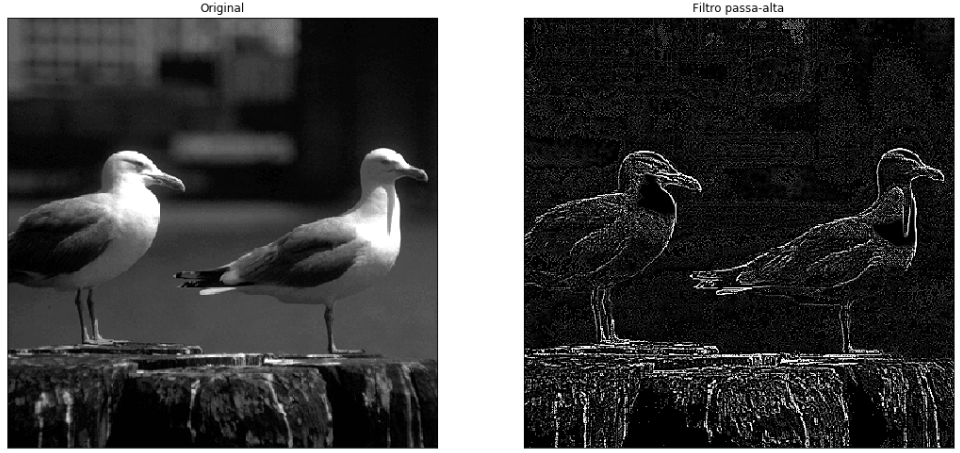
\includegraphics[width=0.99\columnwidth]{pics/high_pass_filter}
	\caption{Resultado da aplicação do filtro passa-alta.\label{fig:filtro-passa-alta}}   
\end{center} 
\end{figure}  

Também percebemos que o resultado do filtro passa-alta realça o ruído na imagem. Podemos atenuar esse problema, aplicando um filtro suavizador (passa-baixa) como um passo anterior. De fato, essa é a proposta do filtro Laplaciano do Gaussiano. No entanto, a intensidade deste filtro deve ser escolhida com cuidado pois, podemos suprimir as regiões de interesse da imagem.

\subsection{Filtro h2}

O próximo filtro, h2, é um filtro Gaussiano com características passa-baixa. Filtros Gaussianos seguem um padrão específico. Eles possuem valores mais acentuados no pixel de referência (pixel central). Porém, a medida que nos distanciamos do pixel central, os valores ficam mais baixos. 

Portanto, a convolução de um filtro Gaussiano em uma imagem é análoga a média ponderada dos pixels em uma vizinhança. A ideia central é que pixels em uma vizinhança mais próxima possuem maior influência no o resultado final do que pixels mais distantes.

Dessa forma, filtros com característica passa-baixa suprimem pixels com intensidades elevadas. Pois esses, serão suavizados pelos valores dos pixels em sua vizinhança (média ponderada). Assim, obtemos o efeito de suavização mostrado na Figure \ref{fig:filtro-passa-baixa}.

\begin{figure}
\begin{center}
	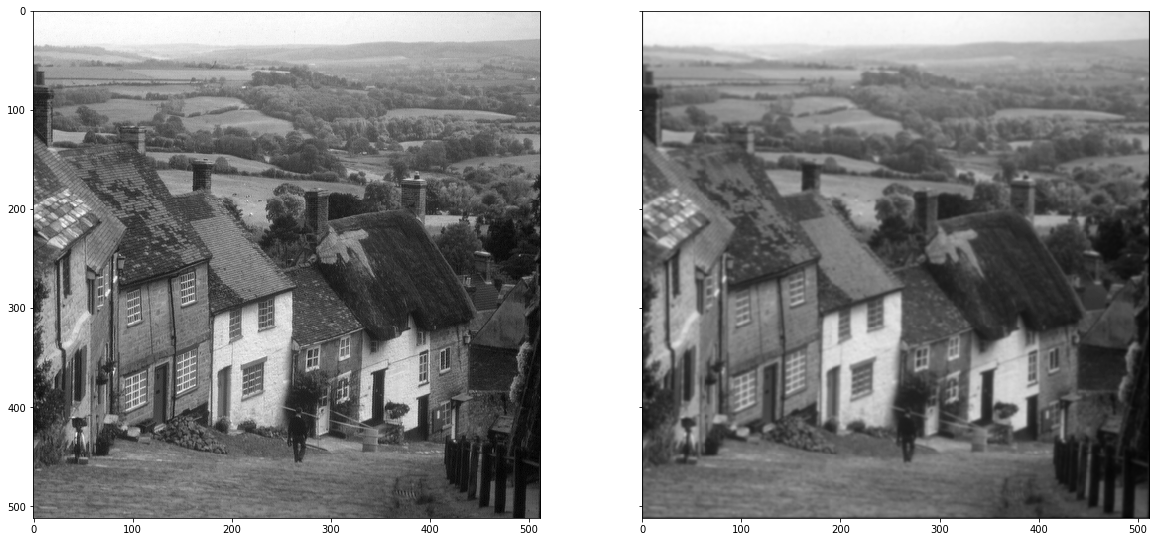
\includegraphics[width=0.99\columnwidth]{pics/gaussian_blur}
	\caption{Resultado da aplicação do filtro passa-baixa Gaussiano.\label{fig:filtro-passa-baixa}}   
\end{center} 
\end{figure}  

\subsection{Filtros h3 e h4}

Para entender a aplicação dos kernels h3 e h4, precisamos nos referir ao conceito de gradiente. Sucintamente, quando lhe damos com funções multivariáveis (como uma imagem), podemos calcular derivadas parciais com relação a cada uma das variáveis. Desta forma, o gradiente é um vetor que encapsula todas as derivadas parciais de uma função. Enquanto derivadas parciais refletem mudanças em direções específicas, o gradiente encapsula taxas de variações em todas as direções. 

No contexto de imagens, a derivada é definida como a subtração dos pixels vizinhos. Esse é o conceito dos filtros passa-alta de Sobel h3 e h4. Quando aplicados h3 e h4 separadamente em uma imagem, nós obtemos a imagem do gradiente. A Figura \ref{fig:sobel} (a) e (b), mostram as derivadas parciais na direção vertical e horizontal respectivamente.

\begin{figure*}[h!]
\begin{center}
	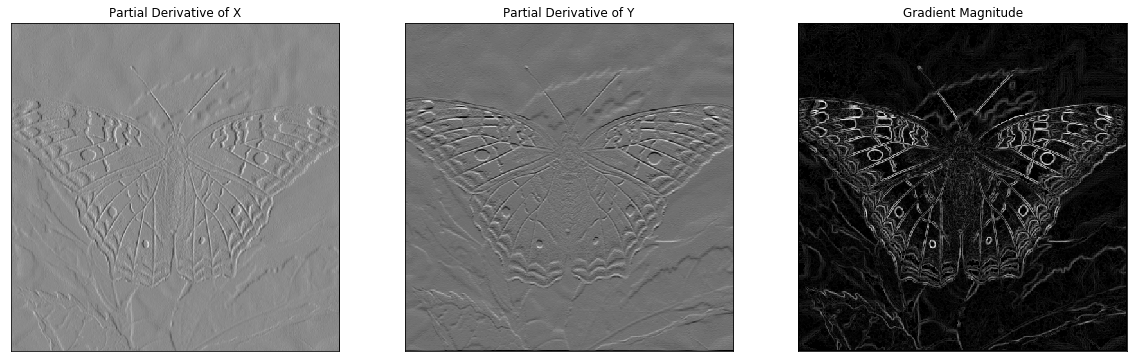
\includegraphics[height=0.67\columnwidth]{pics/sobel}
	\caption{Derivadas parciais nas direções x, y, e magnitude do gradiente calculados com os filtros de Sobel.\label{fig:sobel}}   
\end{center} 
\end{figure*}  

Percebemos que os filtros de Sobel conseguem achar picos nas derivadas (nas duas direções vertical e horizontal). Como as bordas representam as porções da imagem com maior mudança de intensidade (maiores derivadas), os filtros de Sobel enfatizam as bordas de uma imagem.

Finalmente, se calcularmos a magnitude do gradiente, teremos uma imagem de bordas - Figura \ref{fig:sobel} (c).

\section{Notas sobre Implementação}

Dada uma imagem com dimensões $M \times M$, e um filtro com dimensões $N \times N$, uma implementação clássica de convolução necessita de $M^2N^2$ multiplicações e adições. Note que esse é o custo total de convolução do filtro sobre toda a imagem.

No entanto, para \textbf{filtros linearmente separáveis}, (como o filtro Gaussiano e os filtros de Sobel), podemos aproveitar a propriedade de associatividade da convolução e realizar a mesma operação com um ganho significativo de performance.

Filtros linearmente separáveis são filtros que podem ser representados a partir da convolução de um vetor de coluna com o vetor de linha. Dessa forma, ao invés de fazer uma convolução entre uma imagem \textit{f} com um filtro \textit{h}, podemos representar a mesma operação com duas operações de convolução. 

Primeiro, realizamos uma convolução simples verticalmente. Em seguida, aplicamos uma convolução horizontal sobre o resultado anterior. Vide Figura \ref{fig:linear_sep_kernel}. Dessa forma, mesmo utilizado 2 operações de convolução, ao invés de apenas uma, obtemos uma redução no número de operações para $2NM$. Que é algumas ordens de magnitude menor que $N^2M^2$. 

\begin{figure}[h!]
\begin{center}
	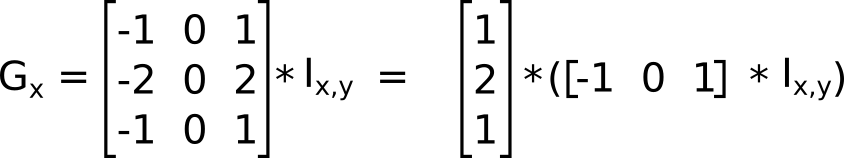
\includegraphics[width=0.99\columnwidth]{pics/linear_sep_kernel}
	\caption{Propriedade de separabilidade linear do filtro de Sobel.\label{fig:linear_sep_kernel}}   
\end{center} 
\end{figure}  

Para a aplicação do filtro Gaussiano e de Sobel implementamos a função \textit{fast\_conv2d()} que implementa convolução com kernels linearmente separaveis. A função utiliza a rotina \textit{convolve(image, kernel)} da biblioteca NumPy.

Observe que a função \textit{convolve(image, kernel)}, implementa uma operação discreta de convolução. Dessa maneira, antes de 'deslizar' o kernel sobre a imagem, \textbf{este é rotacionado em um ângulo de $180º$}. Para kernels simétricos (como o Gaussiano), tal rotação equivale a uma função identidade. No entanto, para kernels não simétricos, como Sobel as duas operações são distintas.

É importante salientar que nossa implementação de \textit{fast\_conv2d()} resolve bordas com padding de zeros (0s). Assim, ao convoluirmos uma imagem com um kernel utilizando \textit{fast\_conv2d()}, obtemos uma outra image com as mesmas dimenssões da imagem de entrada. Na literatura, essa processo é referido como "SAME" padding. Como resultado, convoluções que utilizam "SAME" padding apresentam uma borda escurecida ao redor da imagem.

Para aplicação do kernel h1 (passa-alta), utilizamos a função \textit{filter2D()} do OpenCV. Essa função implementa a operação correlação (não convolução). Porém, como temos um filtro h1 simétrico, as duas operações produzem o mesmo resultado.

%%% Add section %%%%%%%%%%%%%%%%%%%%%%%%%%%%%%%%%%%%%%%%%%%%%%%%%%%%%%%%%%%%%%%%%%
\section{Convolução no Domínio de Frequência}

Uma importante propriedade quando trabalhamos com imagens no domínio de frequência, é que, convolução no domínio espacial é equivalente a multiplicação no domínio de frequência.  Desta forma, dada uma imagem \textit{f} e um kernel gaussiano \textit{h} no domínio espacial, podemos:

\begin{itemize}
	\item Computar a transformada de Fourier para a imagem \textit{f}.
	\item Computar a transformada de Fourier para o filtro Gaussiano \textbf{h}.
	\item Multiplicar os resultados obtidos acima $f \times h$ (Simples multiplicação).
	\item Aplicar a transformada inversa de Fourier para o dominio espacial.
\end{itemize}

A Figure \ref{fig:conv_with_ft} ilustra esse conceito.

\begin{figure}[h!]
\begin{center}
	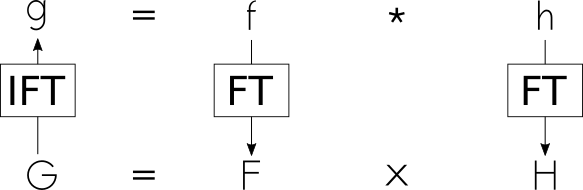
\includegraphics[width=0.99\columnwidth]{pics/ft}
	\caption{Relação entre a operação de convolução no domínio espacial e de frequência.\label{fig:conv_with_ft}}   
\end{center} 
\end{figure} 

Curiosamente, quando aplicamos a Transformada de Fourier (TF) em um kernel Gaussiano, obtemos como resultado outro kernel Gaussiano. No entanto, eles possuem uma caracteristica inversa. Em outras palavras, dado um kernel gaussiano largo (grande sigma) sua TF é uma gaussiana com com um sigma pequeno (gaussiana fina). Analogamente, dado um kernel gaussiano com um sigma pequeno, sua TF resulta em uma gaussiana com um sigma largo. A figura \ref{fig:ft_gaussian} mostra essa relação inversa da gaussiana nos domínios espaciais e de frequência.

\begin{figure}
\begin{center}
	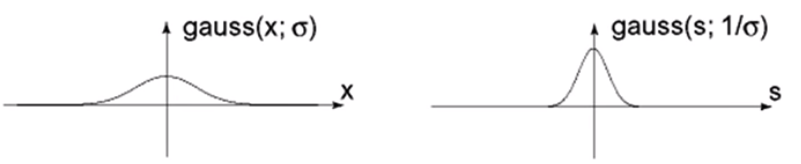
\includegraphics[width=0.99\columnwidth]{pics/ft_gaussian}
	\caption{Resultado da Transformada de Fourier em um kernel Gaussiano.\label{fig:ft_gaussian}}   
\end{center} 
\end{figure} 

A Figura \ref{fig:ft_complete} apresenta os resultados da aplicação do filtro gaussiano em uma imagem no domínio de frequência. A primeira linha mostra como isso é feito no domínio espacial (via convolução), enquanto a segunda linha da figura mostra a mesma operação no domínio de frequência (simples multiplicação).

A Figura \ref{fig:ft_complete} mostra alguns pontos interessantes. Perceba como uma gaussiana com um sigma pequeno, equivale a outra gaussiana com sigma bem maior no domínio de frequência. 

Para criar o kernel gaussiano foi utilizado a função \textit{getGaussianKernel()} do OpenCV. Exploramos os efeitos de vários valores de sigma, por motivos de espaço, apresentamos na Figura \ref{fig:ft_complete} um kernel Gaussiano com sigma 3.

Ao centralizar o espectro da Transformada de Fourier, temos baixa frequência no centro e alta frequência nos arredores. Ao multiplicarmos as duas TF, percebemos na Figura \ref{fig:ft_complete}(f) como o kernel gaussiano mantém as baixas frequências e atenua as altas frequências. Como resultado, obtemos uma imagem suavizada Figura \ref{fig:ft_complete}(c). Optamos por utilizar as rotinas \textit{fft.fft2()}, \textit{fft.fftshift()} e \textit{fft.ifft2()} da biblioteca NumPy para as aplicações descritas acima.

\begin{figure}[h!]
\begin{center}
	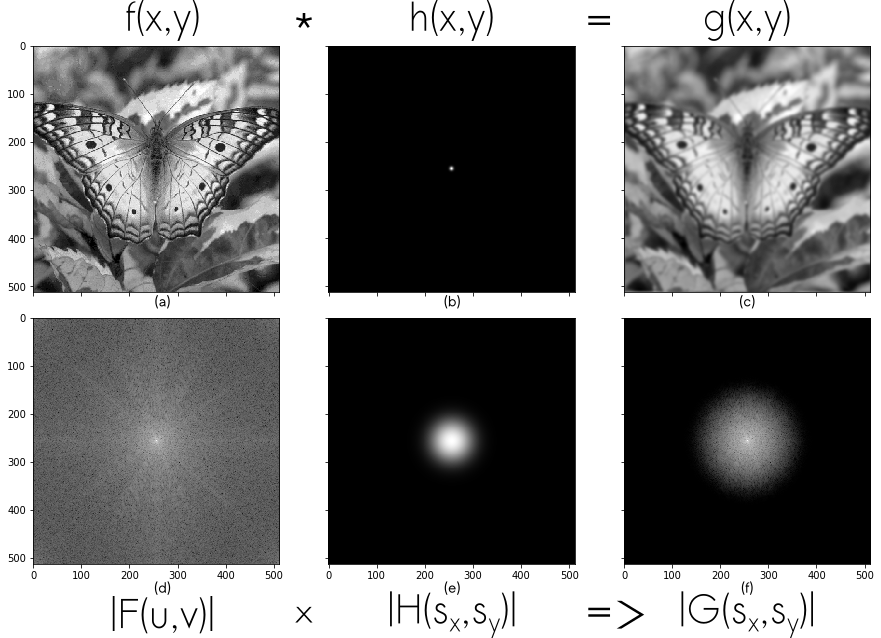
\includegraphics[width=0.99\columnwidth]{pics/ft_complete}
	\caption{Convolução no domínio de frequência com kernel Gaussiano.\label{fig:ft_complete}}   
\end{center} 
\end{figure} 

%\CITEONE{Silva}{Silva_2010} for papers with one author.
%\CITETWO{Silva}{Souza}{Silva_2010b} for papers with two authors.
%\CITEN{Silva}{Silva_2010c} for papers with three or more authors.

%%% Add section %%%%%%%%%%%%%%%%%%%%%%%%%%%%%%%%%%%%%%%%%%%%%%%%%%%%%%%%%%%%%%%%%%
\section{Conclusions and Future Work}

Os resultados do trabalho foram satisfatórios ao que se refere a aplicação de kernels de diversas características nas imagens definidas pelo professor. Investigamos os efeitos de vários limiares (como o valor de sigma para construção das Gaussianas). Exploramos operações de convolução tanto no domínio espacial quanto no de frequência, e enfatizamos as ligações e particularidades entre as duas representações.


%%% References %%%%%%%%%%%%%%%%%%%%%%%%%%%%%%%%%%%%%%%%%%%%%%%%%%%%%%%%%%%%%%%%%%%
{\small
\bibliographystyle{unsrt}
\bibliography{refs}
}


\end{document}